\documentclass{beamer}
\usetheme{Warsaw}
\setbeamertemplate{footline}[frame number]

\usepackage[utf8]{inputenc}
\usepackage{fancybox}
\usepackage{multimedia} 
\usepackage{subfig}
\usepackage{amsmath}
\usepackage{amssymb}

\usepackage{hyperref}
% Setze die Optionen für das hyperref-Paket
\hypersetup{
    colorlinks=true,    % Färbt die Links
    linkcolor=blue,     % Farbe für interne Links
    filecolor=magenta,  % Farbe für Links zu lokalen Dateien
    urlcolor=cyan,      % Farbe für externe Links
    pdftitle={Angewandte Mathematik}, % Titel des Dokuments
    pdfpagemode=FullScreen, % Öffnet das PDF im Vollbildmodus
}

\usepackage[all]{xy}
\usepackage{verbatim}

\begin{document}


\title[Angewandte Mathematik] % (optional, only for long titles)
{Angewandte Mathematik
\\
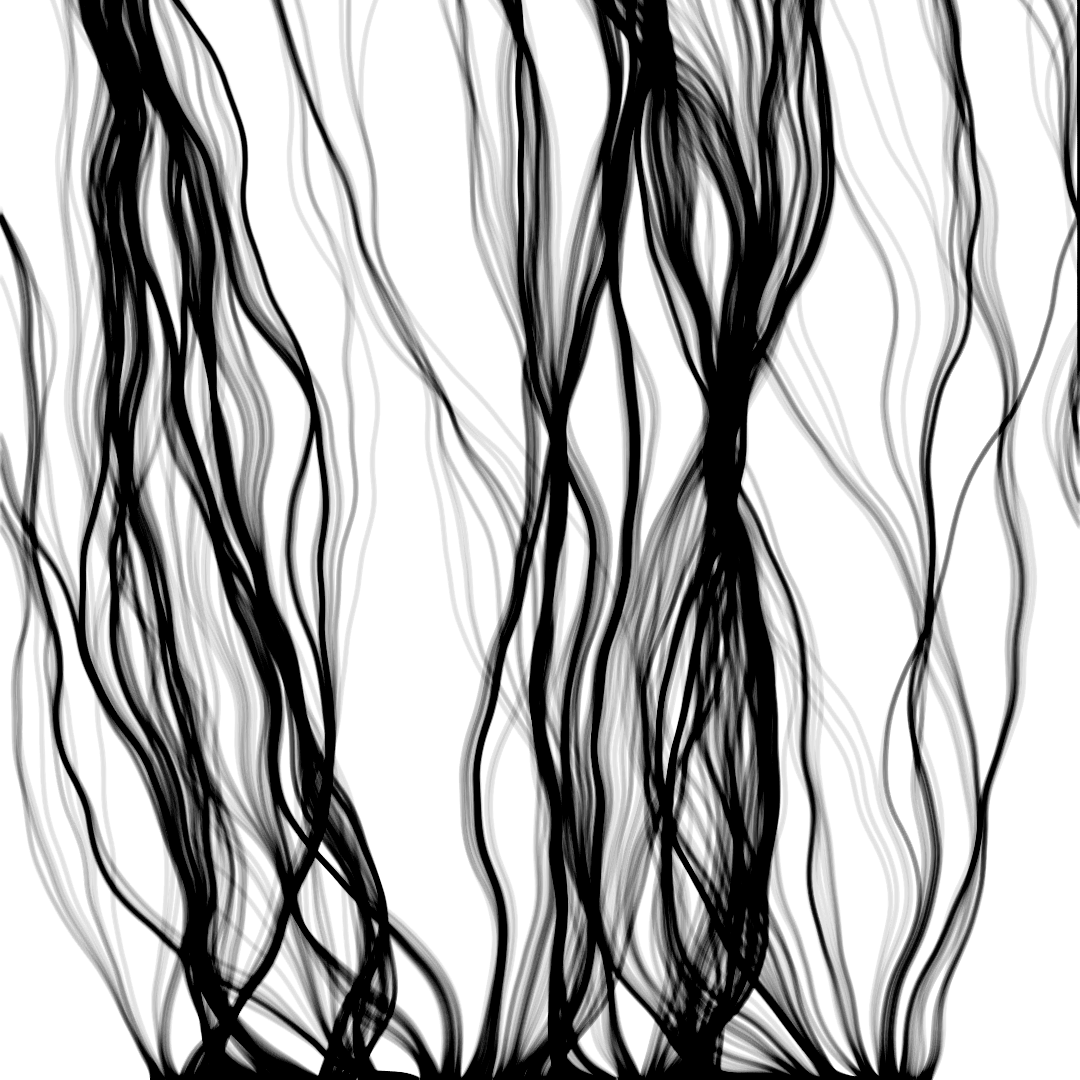
\includegraphics[scale=0.15]{images/cover}
}
\subtitle{}
\author[Dr. Johannes Riesterer] % (optional, for multiple authors)
{Dr.  rer. nat. Johannes Riesterer}

\date[KPT 2004] % (optional)
{}

\subject{Angewandte Mathematik}

\frame{\titlepage}

\begin{frame}
    \frametitle{Angewandte Mathematik}
    \framesubtitle{Asymptotics}
    \begin{block}{Für fast alle (hinreichend große) \href{https://github.com/leanprover-community/mathlib4/blob/418a5eb7aec3fb639097cb13f74fc031ac4057f2/Mathlib/Order/Filter/Defs.lean\#L243-L244}{Mathlib}}
        Für einen Filter $l$ bedeutet die Bedingung 
        \( \forall^f x \;  p(x) \) 
       dass die Menge der Elemente, für die \( p(x) \) gilt, ein Element des Filters \( l \) ist, also
        \( \{ X \; | \;  p(x) \} \in l \).
    \end{block}
\end{frame}

\begin{frame}
    \frametitle{Angewandte Mathematik}
    \framesubtitle{Asymptotics}
    \begin{block}{Big O Notation \href{https://github.com/leanprover-community/mathlib4/blob/69d256b3c87085fec8063376dfb231ee1fd345d8/Mathlib/Analysis/Asymptotics/Asymptotics.lean\#L75-L80}{Mathlib}}
        Für einen Filter $l$ und Funktionen $f,g$ definieren wir 
        \[
       f = \mathcal{O}[l] g \leftrightarrow  \exists c > 0, \forall^\mathsf{f} x \in l, \|f(x)\| \leq c \cdot \|g(x)\|
        \]
    \end{block}

    \begin{block}{Erklärung}
        Die Aussage besagt, dass für fast alle \(x\) in der Menge \(l\), die Norm von \(f(x)\) durch ein Vielfaches der Norm von \(g(x)\) beschränkt ist. Das Vielfache wird durch die Konstante \(c\) dargestellt.
    \end{block}
    
\end{frame}

\begin{frame}
    \frametitle{Angewandte Mathematik}
    \framesubtitle{Asymptotics}

    \begin{block}{Klein-o Notation \href{https://github.com/leanprover-community/mathlib4/blob/69d256b3c87085fec8063376dfb231ee1fd345d8/Mathlib/Analysis/Asymptotics/Asymptotics.lean\#L161-L162}{Mathlib}}
        Für einen Filter $l$ und Funktionen $f,g$ definieren wir 
        \[
       f = o[l] g \leftrightarrow \forall c > 0,  \forall^\mathsf{f} x \in l, \|f(x)\| \leq c \cdot \|g(x)\| \text{ für } x \geq N
        \]
    \end{block}

    \begin{block}{Erklärung}
        Die Aussage besagt, dass für jede positive Konstante \(c\) und für fast alle \(x\) in der Menge \(l\)  die Norm von \(f(x)\) kleiner oder gleich \(c \cdot \|g(x)\|\) ist. Dies beschreibt, dass \(f(x)\) asymptotisch schneller gegen 0 geht als \(g(x)\).
        In anderen Worten, der Ausdruck         
        $\frac{\|f(x)\|}{\|g(x)\|}$
        geht gegen $0$ entlang $l$, wobei mögliche Probleme durch Division durch Null durch diese Definition vermieden werden.
    \end{block}
    
    \begin{block}{Beweis: Klein-o impliziert Groß-O \href{https://github.com/leanprover-community/mathlib4/blob/69d256b3c87085fec8063376dfb231ee1fd345d8/Mathlib/Analysis/Asymptotics/Asymptotics.lean\#L191-L192}{Mathlib}}
        Wenn \( f = o[l] g \), dann ist \( f = O[l] g \).
        \end{block}
    
\end{frame}

\begin{frame}
    \frametitle{Angewandte Mathematik}
    \framesubtitle{Ableitungen}
    \textbf{Klassische Definition in einer Dimension:}
    \[
    f'(a) = \lim_{h \to 0} \frac{f(a + h) - f(a)}{h}
    \]
    
    \textbf{Definition mit \( o \)-Kalkül:}
    \[
    f(a + h) = f(a) + f'(a)h + o(h)
    \]
  
    \textbf{Äquivalenz:} \\
    \vspace{0.2cm}
    1. \textbf{Von \( o(h) \) zur klassischen Definition:} \\
    \quad \( \frac{f(a + h) - f(a)}{h} = f'(a) + \frac{o(h)}{h} \) \\
    \quad Mit \( \lim_{h \to 0} \frac{o(h)}{h} = 0 \) folgt die klassische Definition.
    
    \vspace{0.3cm}
    2. \textbf{Von der klassischen Definition zur \( o(h) \)-Form:} \\
    \quad Nehmen wir \( f'(a) = \lim_{h \to 0} \frac{f(a + h) - f(a)}{h} \), dann: \\
    \quad \( f(a + h) = f(a) + f'(a)h + r(h) \), wobei \( r(h) \) der Restterm ist. \\
    \quad Da \( \lim_{h \to 0} \frac{r(h)}{h} = 0 \), gilt \( r(h) = o(h) \).
    
  \end{frame}
  
  \begin{frame}
    \frametitle{Angewandte Mathematik}
    \framesubtitle{Ableitungen}

\begin{figure}[H]
      \centering
    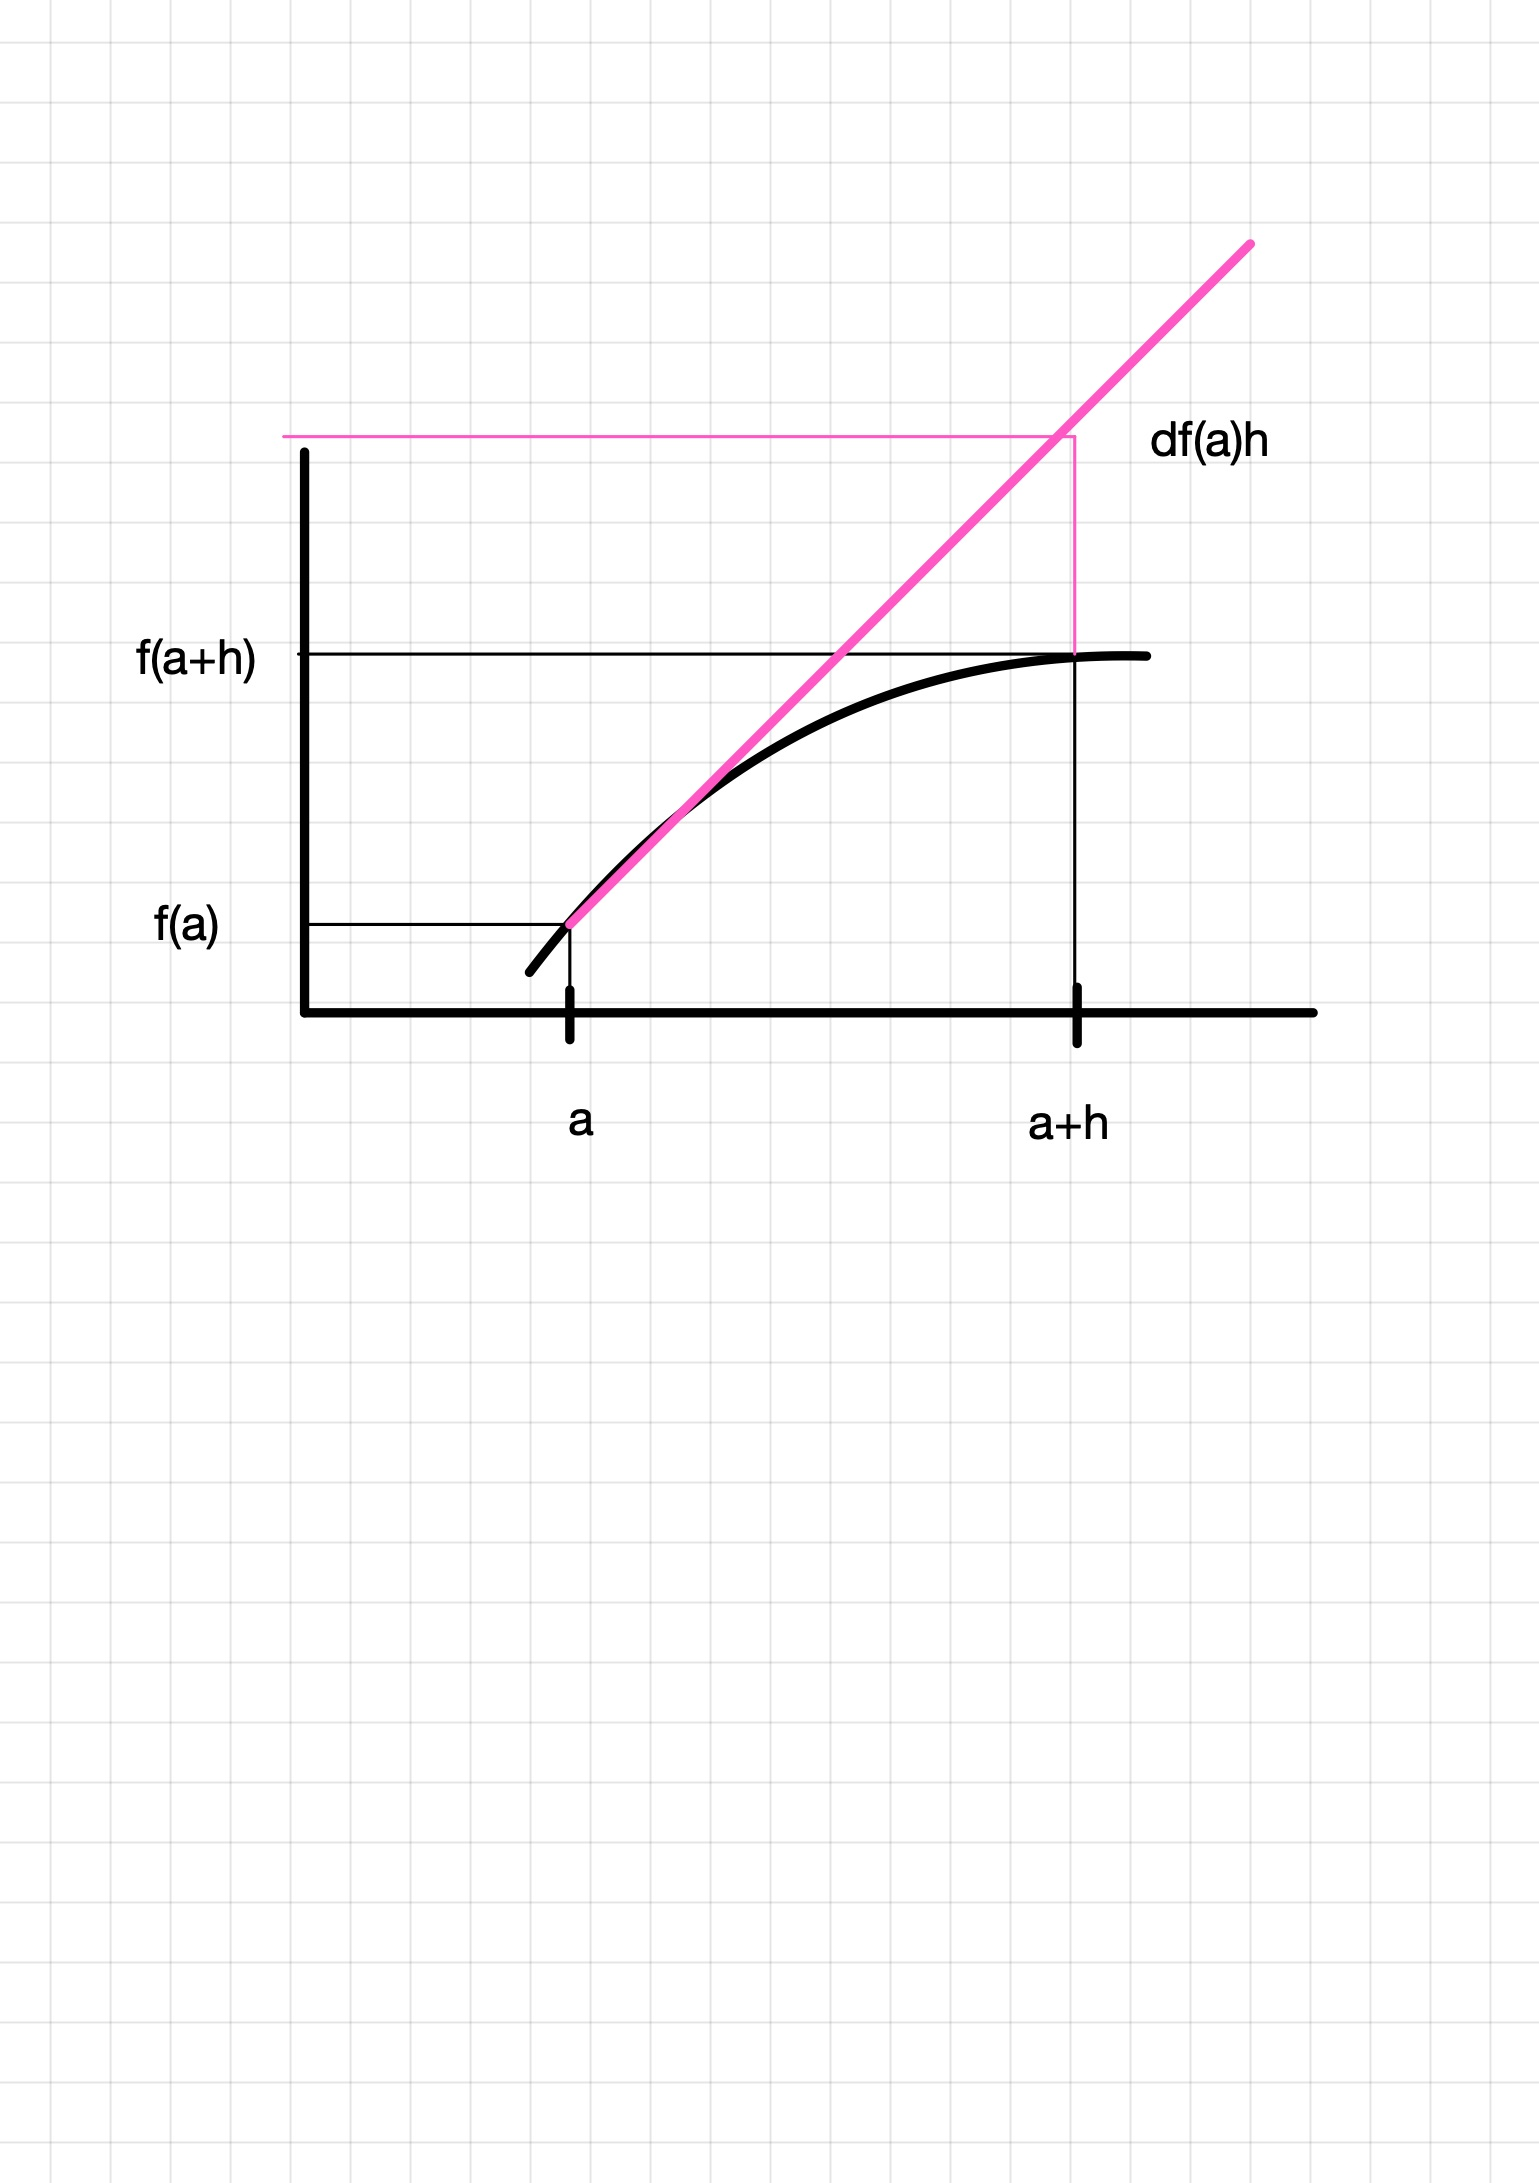
\includegraphics[width=0.8\textwidth]{images/df}
\end{figure}

 \end{frame}


 \begin{frame}
    \frametitle{Angewandte Mathematik}
\framesubtitle{Lokale Linearisierung}
    \begin{block}{Lokale Linearisierung}
Eine Funktion  $f: U \subset \mathbb{R}^n \to \mathbb{R}^m$ heisst differenzierbar  in $a \in U$ falls es eine lineare Funktion 
$df(a):  \mathbb{R}^n \to  \mathbb{R}^m$ gibt mit
\begin{align}
\label{diff}
f(a + h)  =  f(a)  +  df(a) h + o(||h||)  \\
\Leftrightarrow lim_{h \to 0} \frac{f(a + h)  -  f(a)  -  df(a)h}{||h||} = 0
\end{align}
für alle $h \in \mathbb{R}^n$
\end{block}
    \begin{block}{Bedeutung}
Eine differenzierbare Funktion kann  auf hinreichend kleinen Umgebungen 
beliebig genau durch eine lineare Funktion approximiert werden. 
\end{block}
 \end{frame}


 \begin{frame}
    \frametitle{Angewandte Mathematik}
    \framesubtitle{Ableitungen}
    \begin{block}{Beispiel}
$A \in \mathbb{R}^{n \times m}$, $b \in \mathbb{R}^n$ 
\begin{align}
f(x) : = A\cdot x + b \\
df(a) : = A 
\end{align}
\end{block}
    \begin{block}{Beweis}
\begin{align}
& \lim_{h\to 0} \frac{A(x + h) - A\cdot x -A\cdot h}{||h||} = \\
& \lim_{h\to 0} \frac{A\cdot x + A \cdot h - A\cdot x -A\cdot h}{||h||} = 0
\end{align}
\end{block}

 \end{frame}



    \begin{frame}
        \frametitle{Angewandte Mathematik}
        \framesubtitle{Ableitungen}
        \begin{block}{Eindeutigkeit}
    Die Ableitung  $df$ ist eindeutig bestimmt.
    \end{block}
        \begin{block}{Beweis}
    Ist $df'$ eine weiter Abbildung mit Eigenschaft $(\ref{diff})$, so gilt für jeden Basisvektor $e_i$
    \begin{align}
    & \lim_{t \to 0} \frac{f(a+te_i) - f(a) - df(a)t e_i }{||t e_i||} = 0 \\
     & \lim_{t \to 0} \frac{f(a+te_i) - f(a) - df'(a)t e_i }{||t e_i||}  = 0\\
    & \Rightarrow (df(a) - df'(a))(e_i) = lim_{t \to 0}\frac{(df'(a) - df(a))(t e_i)}{||te_i||} = 0
    \end{align}
    \end{block}
     \end{frame}
    


    \begin{frame}
        \frametitle{Lineare Abbildungen}
    
        \begin{block}{Definition}
            Eine Abbildung \( T: V \to W \) zwischen zwei Vektorräumen \( V \) und \( W \) über einem Körper \( K \) heißt \textbf{linear}, wenn für alle \( v_1, v_2 \in V \) und alle \( \alpha, \beta \in K \) gilt:
            \[
            T(\alpha v_1 + \beta v_2) = \alpha T(v_1) + \beta T(v_2).
            \]
        \end{block}
    
        \begin{block}{Eigenschaften}
            \begin{itemize}
                \item Lineare Abbildungen erhalten die Vektorraumstruktur: Sie respektieren die Addition und die Skalarmultiplikation.
                \item Jede lineare Abbildung ist durch ihr Verhalten auf einer Basis des Vektorraums eindeutig bestimmt.
                \item Die Ableitung einer linearen Abbildung ist die Abbildung selbst: Für eine lineare Abbildung \( T \) gilt \( D(T) = T \).
            \end{itemize}
        \end{block}
    
  
        
    \end{frame}
    
    \begin{frame}
        \frametitle{Lineare Abbildungen}
    
    
        \begin{block}{Beispiele}
            \begin{itemize}
                \item Die Identitätsabbildung \( \text{id}_V: V \to V \), definiert durch \( \text{id}_V(v) = v \), ist linear.
                \item Projektionen und Rotationen in \( \mathbb{R}^n \) sind lineare Abbildungen.
                \item Matrizen wirken als lineare Abbildungen auf Vektorräumen.
            \end{itemize}
        \end{block}
        
    \end{frame}
    

    \begin{frame}
        \frametitle{Angewandte Mathematik}
        \framesubtitle{Ableitungen}
        \begin{block}{Partielle Ableitung}
            In Lean4 (Mathlib) wird eine lineare Abbildung \( T \) zwischen zwei normierten Vektorräumen \( V \) und \( W \) über \( \mathbb{R} \) als eine stetige lineare Abbildung (\texttt{continuous\_linear\_map}) definiert:
            \[
            T : V \to L[\mathbb{R}] W
            \]
            Die lineare Struktur wird durch zwei Eigenschaften beschrieben:
            \begin{itemize}
                \item \texttt{map\_add : $T (v_1 + v_2) = T v_1 + T v_2$}
                \item \texttt{map\_smul : $T (c \cdot v) = c \cdot T v$}
            \end{itemize}
        \end{block}
    
    \end{frame}


\begin{frame}
    \frametitle{Angewandte Mathematik}
    \framesubtitle{Ableitungen}

\begin{block}{Definition}
  Eine Funktion \( f \) ist an \( x \) differenzierbar, wenn:
  \[
  f(x') - f(x) - f'(x' - x) = o[L](x' - x)
  \]
  Dies bedeutet, dass der Restterm \( f(x') - f(x) - f'(x' - x) \) schneller gegen 0 geht als \( x' - x \), wenn \( x' \to x \) unter einem Filter \( L \).
\end{block}

\begin{block}{Beispiele für Filter \( L \)}
  \begin{itemize}
    \item \textbf{Standardfall: Filter der Umgebung von \( x \)} \\
    Der Filter \( L = \mathcal{N}(x) \) beschreibt, dass \( x' \) beliebig nahe an \( x \) heranrückt. Dieser Filter erfasst alle offenen Umgebungen von \( x \). 
    \[
    o[{\mathcal{N}(x)}](x' - x)
    \]
    bedeutet, dass der Restterm verschwindet, wenn \( x' \) gegen \( x \) läuft.
  \end{itemize}
\end{block}
\end{frame}

\begin{frame}
    \frametitle{Angewandte Mathematik}
    \framesubtitle{Ableitungen}

\begin{block}{Beispiele für Filter \( L \) (Fortsetzung)}
  \begin{itemize}
      
    \item \textbf{Filter auf einem Teilraum:} \\
    Wenn man Differenzierbarkeit nur auf einem Teilraum \( S \subseteq E \) betrachtet, 
    verwendet man den Filter \( \mathcal{N}[S](x) \), der Umgebungen in \( S \) enthält. Damit kann man die Differenzierbarkeit von \( f \) auf \( S \) testen.
  
    \item \textbf{Filter für gerichtete Mengen:} \\
    Bei Funktionen auf gerichteten Mengen (z.B. in Optimierungsproblemen) verwendet man den Filter \( L \), der beschreibt, wie \( x' \) sich entlang einer Richtung oder eines Pfades \( \gamma(t) \to x \) nähert.
  \end{itemize}
\end{block}

\vspace{-0.5cm} % Adjust spacing to avoid overfull vbox

\begin{block}{Zusammenfassung}
  Der Filter \( L \) gibt die Art und Weise an, wie \( x' \) gegen \( x \) strebt. Der häufigste Fall ist der Filter der offenen Umgebungen von \( x \), aber auch Teilräume oder spezielle Pfade können durch Filter modelliert werden.
\end{block}

\end{frame}



\begin{frame}
    \frametitle{Angewandte Mathematik}
    \framesubtitle{Ableitungen}

    \begin{block}{Definition in Lean (Mathlib)}
        In Lean4 (Mathlib) wird eine lineare Abbildung \( T \) zwischen zwei normierten Vektorräumen \( V \) und \( W \) über \( \mathbb{R} \) als eine stetige lineare Abbildung (\texttt{continuous\_linear\_map}) definiert:
        \[
        T : V \to L[\mathbb{R}] W
        \]
        Die lineare Struktur wird durch zwei Eigenschaften beschrieben:
        \begin{itemize}
            \item \texttt{map\_add : $T (v_1 + v_2) = T v_1 + T v_2$}
            \item \texttt{map\_smul : $T (c \cdot v) = c \cdot T v$}
        \end{itemize}
    \end{block}

    \begin{block}{Vergleich}
       Im endlichdimensionalen Fall entspricht die Definition in Lean der üblichen Definition einer linearen Abbildung. 
       Im unendlichdimensionalen Fall wird zusätzlich die Stetigkeit gefordert, da diese nicht automatisch gegeben ist.
    \end{block}
    
\end{frame}

    \begin{frame}
        \frametitle{Angewandte Mathematik}
        \framesubtitle{Ableitungen}
        \begin{block}{Ableitung Berechnen}
            Wie kann man die Ableitung einer Funktion berechnen?
        \end{block}
    
    \end{frame}




    \begin{frame}
        \frametitle{Angewandte Mathematik}
        \framesubtitle{Ableitungen}  
        \begin{block}{Partielle Ableitung}
            Für eine Funktion $f: \mathbb{R}^n \to \mathbb{R}$ definert man die partielle Ableitung 
            \[
                D_i f (x) = \lim_{h \to 0} \frac{f(x + h \cdot e_i) - f(x)}{h}
                \]
            wobei \( e_i \) der \( i \)-te Einheitsvektor ist. 
           
            \( \frac{\partial f(x)}{\partial x_i} :=  D_i f (x)\).
            
        \end{block}

        \begin{block}{Richtungsableitung}
            Allgemeiner definiert man für $f: \mathbb{R}^n \to \mathbb{R}$ und  $v \in \mathbb{R}^n$
            \[
                D_v f (x) = \lim_{h \to 0} \frac{f(x + h \cdot v) - f(x)}{h}
                \]
            die Richtungsableitung von $f$ an der Stelle $x$ in Richtung $v$.            
        \end{block}
    \end{frame}

    \begin{frame}
        \frametitle{Angewandte Mathematik}
        \framesubtitle{Ableitungen}  
    
    \begin{figure}[H]
          \centering
        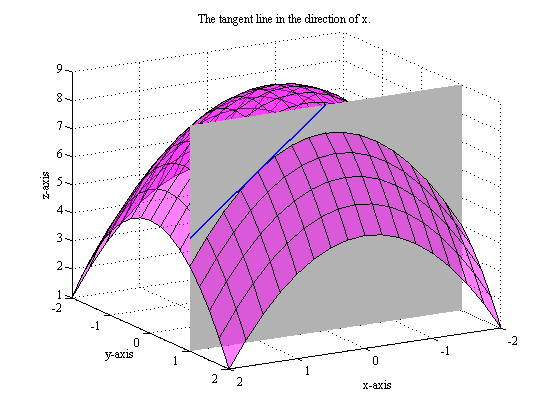
\includegraphics[width=0.95\textwidth]{images/diffable}
    \end{figure}
    
     \end{frame}





     \begin{frame}
        \frametitle{Angewandte Mathematik}
        \framesubtitle{Ableitungen}

    \framesubtitle{Differenzierbarkeit}
        \begin{block}{Gradient}
    
    Der Vektor 
    $$\nabla f (a) := \begin{pmatrix}  \frac{\partial f(a)}{\partial x_1} \\  \vdots \\ \frac{\partial f(a)}{\partial x_n}  \end{pmatrix}$$
    wird als Gradient bezeichnet. 
    \end{block}
    \begin{figure}[H]
          \centering
        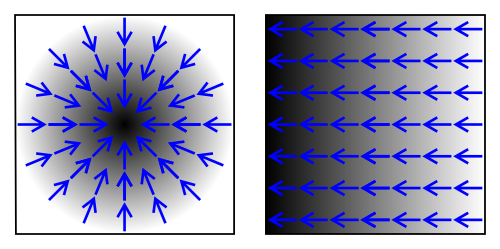
\includegraphics[width=0.7\textwidth]{images/Gradient}
          \caption{Quelle: Wikipedia: https://commons.wikimedia.org/wiki/File:Gradient2.svg}
    \end{figure}
    
    
     \end{frame}
    

 % Folie 1: Einfache Beispiele für den Gradienten
\begin{frame}{Gradienten-Beispiele: Einfache Funktionen}

    \textbf{Beispiel 1: Quadratische Funktion in 2D}
    \[
    f(x, y) = x^2 + y^2
    \]
    Gradient:
    \[
    \nabla f(x, y) = 
    \begin{pmatrix}
    \frac{\partial f}{\partial x} \\
    \frac{\partial f}{\partial y}
    \end{pmatrix}
    = 
    \begin{pmatrix}
    2x \\
    2y
    \end{pmatrix}
    \]
    
    \textbf{Beispiel 2: Quadratische Funktion in 3D}
    \[
    f(x, y, z) = x^2 + y^2 + z^2
    \]
    Gradient:
    \[
    \nabla f(x, y, z) = 
    \begin{pmatrix}
    \frac{\partial f}{\partial x} \\
    \frac{\partial f}{\partial y} \\
    \frac{\partial f}{\partial z}
    \end{pmatrix}
    = 
    \begin{pmatrix}
    2x \\
    2y \\
    2z
    \end{pmatrix}
    \]
    
    \end{frame}
    
    % Folie 2: Komplexere Beispiele für den Gradienten
    \begin{frame}{Gradienten-Beispiele: Komplexere Funktionen}
    
    \textbf{Beispiel 3: Exponentialfunktion}
    \[
    f(x, y) = e^{x^2 + y^2}
    \]
    Gradient:
    \[
    \nabla f(x, y) = 
    \begin{pmatrix}
    \frac{\partial}{\partial x} e^{x^2 + y^2} \\
    \frac{\partial}{\partial y} e^{x^2 + y^2}
    \end{pmatrix}
    = 
    \begin{pmatrix}
    2x e^{x^2 + y^2} \\
    2y e^{x^2 + y^2}
    \end{pmatrix}
    \]
    
    \textbf{Beispiel 4: Logarithmische Funktion}
    \[
    f(x, y) = \ln(x^2 + y^2)
    \]
    Gradient:
    \[
    \nabla f(x, y) = 
    \begin{pmatrix}
    \frac{\partial}{\partial x} \ln(x^2 + y^2) \\
    \frac{\partial}{\partial y} \ln(x^2 + y^2)
    \end{pmatrix}
    = 
    \begin{pmatrix}
    \frac{2x}{x^2 + y^2} \\
    \frac{2y}{x^2 + y^2}
    \end{pmatrix}
    \]
    
    \end{frame}
    

         
    \begin{frame}
        \frametitle{Vergleich: Lineare Abbildungen in Mathematik und Lean (Mathlib)}
        
        
        \begin{block}{Richtungsableitungv und Ableitung}
            \[
                D_v f (x) = df(x) v
            \]
            und damit insbesondere  $df(a) \cdot h = \langle \nabla f (a) , h \rangle$.
        \end{block}

        \begin{block}{Beweisg}
            Folgt aus der Eindeutigkeit der Ableitung.
        \end{block}
    \end{frame}

    


    \begin{frame}{Ziel: Linienableitung innerhalb einer Menge zeigen}
        \begin{block}{Lemma: HasFDerivWithinAt.hasLineDerivWithinAt}
            Wenn \( f \) an \( x \) innerhalb der Menge \( s \) differenzierbar ist mit Ableitung \( L \), dann hat \( f \) eine Richtungsableitung (Linienableitung) in Richtung \( v \), die durch \( L(v) \) gegeben ist:
            \[
            \text{HasFDerivWithinAt } f \, L \, s \, x \Rightarrow \text{HasLineDerivWithinAt } \mathbb{K} \, f \, (L(v)) \, s \, x \, v.
            \]
        \end{block}
    \end{frame}
    
    \begin{frame}{Beweisschritte: Definition der Hilfsfunktion \( F \)}
        \begin{block}{1. Definition einer Hilfsfunktion \( F \)}
            Um die Richtungsableitung in Richtung \( v \) zu bestimmen, definieren wir die Funktion
            \[
            F(t) := x + t \cdot v.
            \]
            Damit repräsentiert \( F \) eine Bewegung entlang der Richtung \( v \) vom Punkt \( x \) aus.
        \end{block}
    
        \begin{block}{2. Darstellung von \( x \) durch \( F \)}
            Wir erkennen, dass \( x = F(0) \), also der Punkt \( x \) durch die Funktion \( F \) bei \( t = 0 \) beschrieben werden kann. Dies verwenden wir, um \( x \) im Beweis durch \( F(0) \) zu ersetzen:
            \[
            \text{rewrite: } x = F(0) \text{ in } \texttt{hf}.
            \]
        \end{block}
    \end{frame}
    
    \begin{frame}{Beweisschritte: Berechnung der Ableitung von \( F \)}
        \begin{block}{3. Ableitung von \( F \) innerhalb der Menge \( s \)}
            Da \( F(t) = x + t \cdot v \), können wir die Ableitung von \( F \) an \( t = 0 \) innerhalb der Menge \( F^{-1}(s) \) berechnen. Diese Ableitung ist:
            \[
            \text{HasDerivWithinAt } F \, (0 + 1 \cdot v) \, (F^{-1}(s)) \, 0.
            \]
            Diese Ableitung resultiert aus der Kombination der konstanten Funktion \( x \) und der Identitätsfunktion, multipliziert mit \( v \).
        \end{block}
    
        \begin{block}{4. Vereinfachung der Ableitung}
            Die Berechnung vereinfacht sich zu:
            \[
            \text{HasDerivWithinAt } F \, v \, (F^{-1}(s)) \, 0.
            \]
            durch die Gleichungen \( 1 \cdot v = v \) und \( 0 + v = v \).
        \end{block}
    \end{frame}
    
    \begin{frame}{Schlussfolgerung: Richtungsableitung von \( f \) entlang \( v \)}
        \begin{block}{5. Kombination der Ableitungen}
            Mit der Kettenregel schließen wir, dass die Richtungsableitung von \( f \) in Richtung \( v \) durch \( L(v) \) gegeben ist:
            \[
            \text{HasLineDerivWithinAt } \mathbb{K} \, f \, (L(v)) \, s \, x \, v.
            \]
            Dies zeigt, dass die Ableitung von \( f \) in Richtung \( v \) der Anwendung von \( L \) auf \( v \) entspricht.
        \end{block}
    \end{frame}



    
    \begin{frame}
        \frametitle{Mehrdimensionale Differentialrechnung}
    \framesubtitle{Differenzierbarkeit}
        \begin{block}{Gradient}
    
    Sei   $f: U \to \mathbb{R}$ differenzierbare Funktion,  $a \in U$ und $v := \text{argmax}_{ ||h|| = 1 } \{ \partial_h f(a) \}$.
    Dann gilt 
    \begin{align*}
    || \nabla f(a) || v =  \nabla f(a) \; .
    \end{align*} 
    \end{block}
    \begin{block}{Gradient}
    Der Gradient zeigt in die Richtung des steilsten Anstiegs.
    \end{block}
    
     \end{frame}
    
    \begin{frame}
        \frametitle{Mehrdimensionale Differentialrechnung}
    \framesubtitle{Differenzierbarkeit}
        \begin{block}{Beweis}
    Für beliebiges $h$ gilt 
    \begin{align*}
    \partial_h f(a) = df(a) h = \langle \nabla f(a) , h \rangle = || \nabla f(a)||  \cdot ||h|| \cdot \cos(\varphi) 
    \end{align*} 
    wobei $\varphi$ den Innenwinkel zwischen $\nabla f(a)$ und $h$ bezeichnet. Für $||h|| = 1$ wird somit $\partial_h f(a) $ maximal, wenn $\varphi = 0$ und somit$h =  \frac{\nabla f(a)}{||\nabla f(a)||}$ ist.
    \end{block}
    
     \end{frame}
    



\begin{frame}
    \frametitle{Angewandte Mathematik}
\framesubtitle{Extrema}
    \begin{block}{Extrema}
Sei $f : X \subset \mathbb{R}^n \to \mathbb{R}$ eine relle Funktion.  Ein Punkt $a \in  X$ heißt lokales Maximum bzw. Minimum, falls eine Umgebung $U$ von $a$ existiert, so dass $f(x) \leq f(a)$ bzw.  $f(x) \geq f(a)$ für alle $x \in U$ gilt. Liegt einer der beiden Fälle vor, so spricht man von einem lokalen Extremum. Gilt strikt $f(x) <  f(a)$ bzw.  $f(x) > f(a)$ , so nennt man das Extremum isoliert. Ist $U = X$ so nennt man es auch globales Maximum bzw. Minimum.
\end{block}
 \end{frame}


\begin{frame}
    \frametitle{Angewandte Mathematik}
\framesubtitle{Extrema}

\begin{figure}[H]
      \centering
    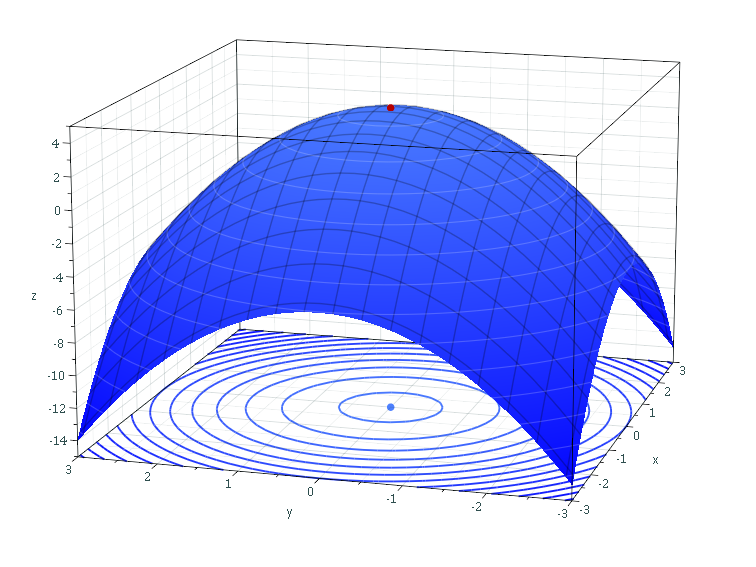
\includegraphics[width=0.8\textwidth]{images/MaximumParaboloid}
      \caption{Quelle: Wikipedia: https://en.wikipedia.org/wiki/File:MaximumParaboloid.png}
   \end{figure}
 \end{frame}

\begin{frame}
    \frametitle{Angewandte Mathematik}
\framesubtitle{Extrema}

\begin{figure}[H]
      \centering
    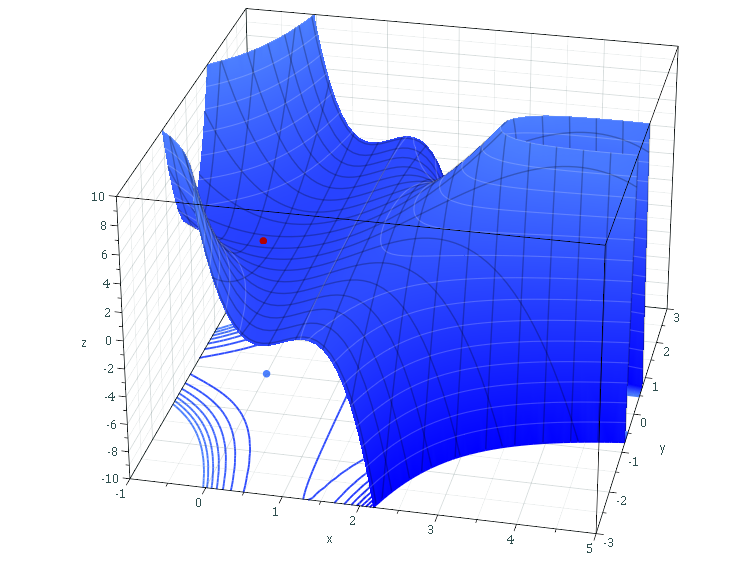
\includegraphics[width=0.8\textwidth]{images/MaximumCounterexample}
      \caption{Quelle: Wikipedia: https://en.wikipedia.org/wiki/File:MaximumCounterexample.png}
\end{figure}
 \end{frame}



\begin{frame}
    \frametitle{Angewandte Mathematik}
\framesubtitle{Extrema}
    \begin{block}{Extrema}
 Ist $f: U  \to \mathbb{R}$ differenzierbar und hat  $f$ in $a \in U$ ein lokales Extremum, so gilt 
\begin{align*}
\frac{\partial}{\partial x_{1}} f(a) = \cdots  = \frac{\partial}{\partial x_{n}} f(a) = 0 \;.
\end{align*}
Sind die partiellen Ableitungen stetig, ist dies  gleichbedeutend mit $df(a) = 0$.
\end{block}
    \begin{block}{Kritischer Punkt}
 Ein Punkt $a$ mit $df(a) = 0$ wird kritischer Punkt genannt.
\end{block}

 \end{frame}

\begin{frame}
    \frametitle{Angewandte Mathematik}
\framesubtitle{Extrema}
    \begin{block}{Beweis}
Setze $F_k(t) := f(a + t e_k)$. Da $f$ ein Extremum in $a$ hat, hat $F_k$ in einer hinreichend kleinen Umgebung um $0$ ein Extremum. 
Da $F_k$ eine Funktion einer Veränderlichen ist, gilt $F'(0) = 0$. Da $\frac{\partial}{\partial x_k} f(a) = F_k'(0)$ folgt die Behauptung.
\end{block}
 \end{frame}







 \begin{frame}{Zielsetzung: Filterdifferenzierbarkeit der Komposition}
    \begin{block}{Theorem (Filterdifferenzierbarkeit der Komposition)}
        Gegeben seien differenzierbare Funktionen \( f : E \rightarrow F \) und \( g : F \rightarrow G \) mit
        \[
        f'(x) : E \to F \quad \text{und} \quad g'(f(x)) : F \to G,
        \]
        wobei \( f'(x) \) und \( g'(f(x)) \) die Ableitungen von \( f \) bzw. \( g \) an den jeweiligen Punkten darstellen.

        Dann ist die Komposition \( h = g \circ f \) differenzierbar und die Ableitung \( h'(x) \) gegeben durch:
        \[
        h'(x) = g'(f(x)) \circ f'(x).
        \]
    \end{block}
\end{frame}

\begin{frame}{Schritte des Beweises in klassischer Mathematik}
    \begin{block}{1. Definition des Fehlerterms für \( f \)}
        Da \( f \) an \( x \) differenzierbar ist:
        \[
        f(y) = f(x) + f'(x)(y - x) + o(\| y - x \|),
        \]
        wobei der Fehlerterm \( o(\| y - x \|) \) schneller gegen Null geht als \( \| y - x \| \).
    \end{block}

    \begin{block}{2. Definition des Fehlerterms für \( g \)}
        Da \( g \) an \( f(x) \) differenzierbar ist:
        \[
        g(f(y)) = g(f(x)) + g'(f(x))(f(y) - f(x)) + o(\| f(y) - f(x) \|).
        \]
    \end{block}
\end{frame}

\begin{frame}{Kombinieren der Fehlerterme}
    \begin{block}{3. Einsetzen des Fehlers von \( f \) in den Fehler von \( g \)}
        Ersetzen von \( f(y) - f(x) \) durch den Ausdruck aus Schritt 1 ergibt:
        \begin{align*}
        g(f(y)) = g(f(x)) + g'(f(x))\left(f'(x)(y - x)  + o(\| y - x \|)\right)  \\ 
        + o(\| f(y) - f(x) \|).
    \end{align*}
\end{block}

    \begin{block}{4. Vereinfachen und Abschätzen}
        Da die Terme \( g'(f(x))(o(\| y - x \|)) \) und \( o(\| f(y) - f(x) \|) \) gegen Null gehen, ist
        \[
        h(y) = h(x) + h'(x)(y - x) + \text{Fehlerterm},
        \]
        was die Differenzierbarkeit von \( h = g \circ f \) zeigt.
    \end{block}
\end{frame}



\begin{frame}{Verbindung zwischen klassischem Beweis und Lean-Code}
    \begin{block}{Schritt-für-Schritt-Übersetzung}
        \begin{itemize}
            \item \texttt{hg : HasFDerivAtFilter g g' (f x) L'} und \texttt{hf : HasFDerivAtFilter f f' x L} entsprechen den Differenzierbarkeitsannahmen von \( g \) und \( f \).
            \item \texttt{eq\(_1\)} und \texttt{eq\(_2\)} repräsentieren die asymptotischen Abschätzungen, die den klassischen Fehlertermen entsprechen.
            \item \texttt{refine .of\_isLittleO <| eq\(_2\).triangle <| eq\(_1\).congr\_left} verwendet die Dreiecksungleichung und die \( o(\cdot) \)-Schranken, um die Differenzierbarkeit zu folgern.
        \end{itemize}
    \end{block}
\end{frame}

\end{document}
